%!TEX root = paper.tex

\section{Markov-Chain Monte Carlo}\label{sec:mcmc}

To evaluate the quality of the covariance estimates produced by our method, we used Markov-Chain Monte Carlo (MCMC) as a benchmark for the ``true'' distribution of the logistic regression weights $(w_0, w_1, w_2)$.  We used the \texttt{R} package \texttt{MCMCpack} with an improper uniform prior, 10,000 iterations, and burn-in rate of 1,000 iterations.  We also compared to
an MCMC simulation with a normal prior on the weights $\mathcal{N}(\M{0},1000I)$ and found similar results. Figures~\ref{fig:mcmc_iterations} and \ref{fig:mcmc_iterations_normal} show the progression of the MCMC algorithm assuming each prior.  

\begin{figure}
\centering
	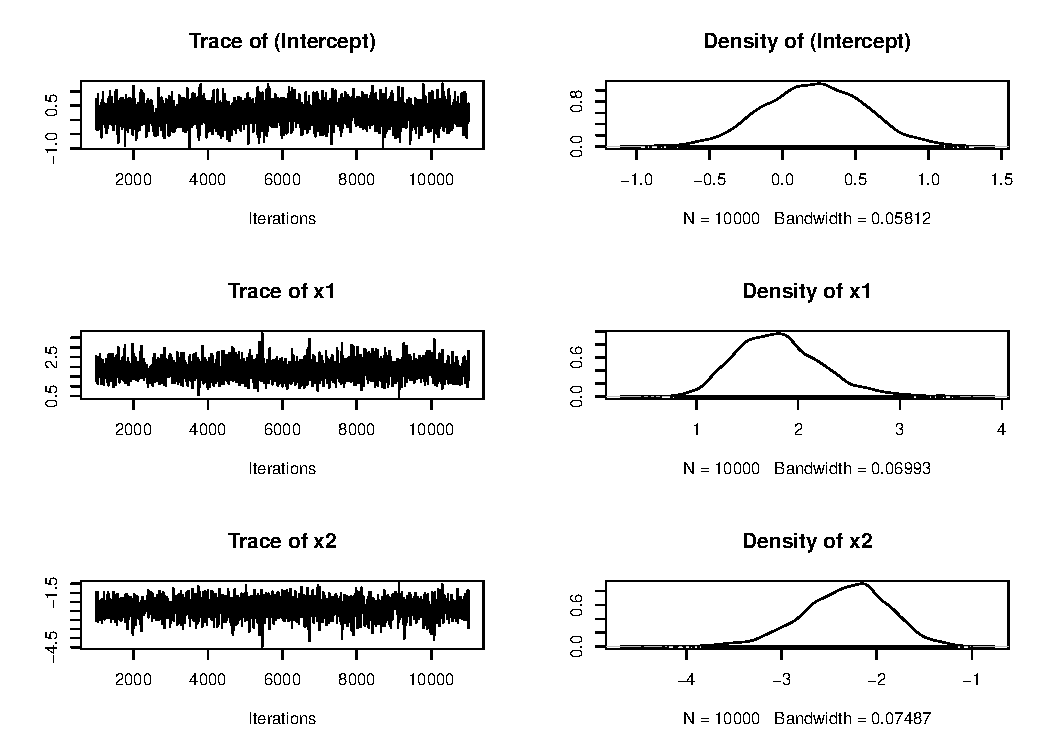
\includegraphics[height=100mm]{figures/mcmc_uniform.pdf}
    \caption{MCMC simulations of logistic regression weights for Dataset 0, and corresponding marginal density plots, assuming 
    an improper uniform prior. 10,000 iterations total.}  \label{fig:mcmc_iterations}  
\end{figure}

\begin{figure}
\centering
	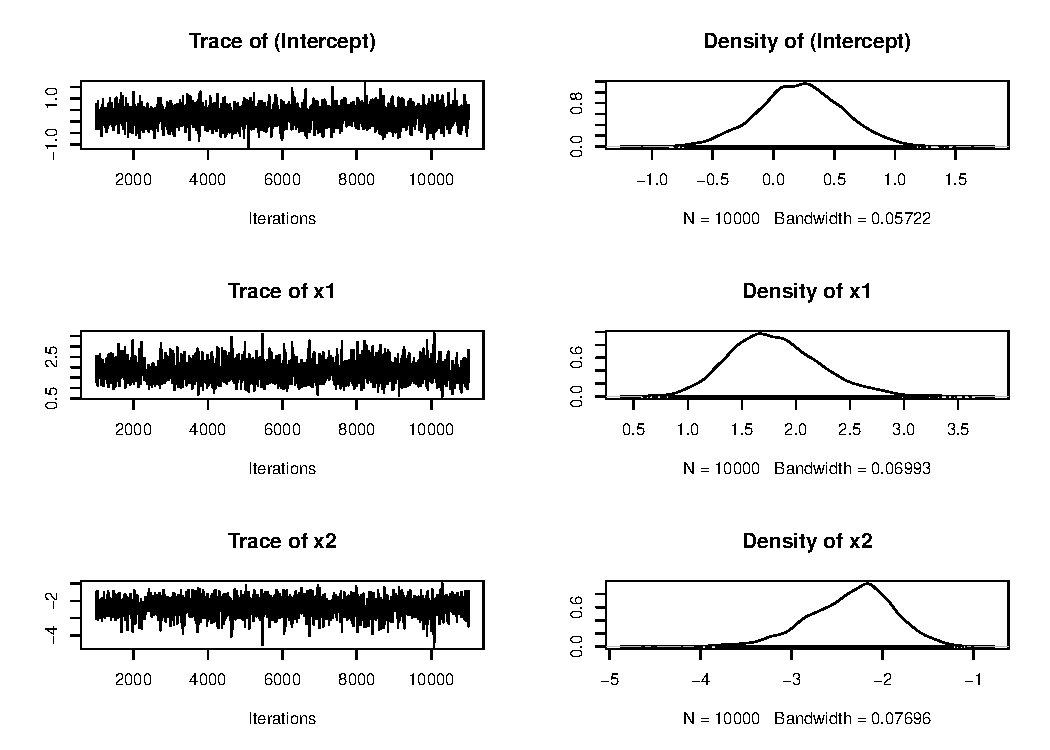
\includegraphics[height=100mm]{figures/mcmc_normal.pdf}
    \caption{MCMC simulations of logistic regression weights for Dataset 0, and corresponding marginal density plots, assuming 
    a normal prior $\mathcal{N}(\M{0},1000I)$. 10,000 iterations total.}  \label{fig:mcmc_iterations_normal}  
\end{figure}

To visualize the joint distribution of the logistic regression weights, we plot the MCMC results for the values of $w_1$ and $w_2$.  In addition, we fit a kernel density to the MCMC simulated weights as a proxy for the contour plot of this empirical distribution, using the \texttt{R} package \texttt{MASS}, which is shown in Figure~\ref{fig:mcmc_kernel}.  

In order to evaluate the accuracy of the covariance matrix of $\M{w}$ given by MFVB logistic regression, which is 3-dimensional, we overlay its contour plot with the MCMC kernel density plot, for Dataset 0 along the dimensions of $w_1$ and $w_2$.  The contour plot of MFVB logistic regression for the logistic regression weights is bivariate normal $\mathcal{N}(\M{\tilde w},\M{\tilde V})$, where $\M{\tilde w},\M{\tilde V}$ are the MFVB parameters excluding the components involving $w_0$.  Figure~\ref{fig:mcmc_mfvb} shows the contour plot of MFVB and the kernel density of MCMC on Dataset 0.  Since MFVB is known to underestimate the covariance of the underlying distribution, we expect the kernel density of MCMC to be more spread out than the contour plot of MFVB logistic regression, which is what we observe.  

\begin{figure}
\centering
	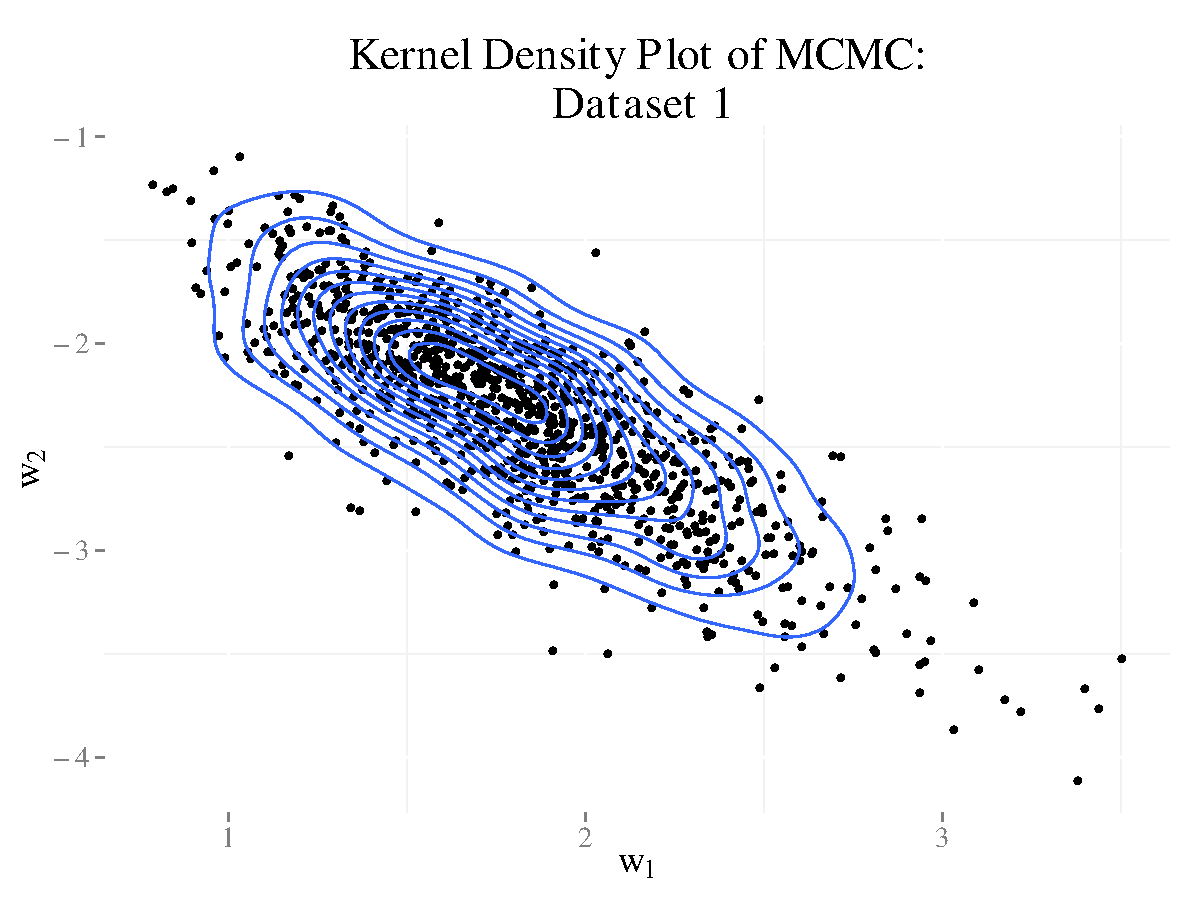
\includegraphics[height=100mm]{figures/mcmc_uniform_2d.pdf}
    \caption{MCMC simulations of logistic regression weights for Dataset 0, and corresponding kernel density plot, assuming 
    an improper uniform prior.  Subset of 1,000 out of 10,000 total iterations shown.}  \label{fig:mcmc_kernel}  
\end{figure}

\begin{figure}
\centering
	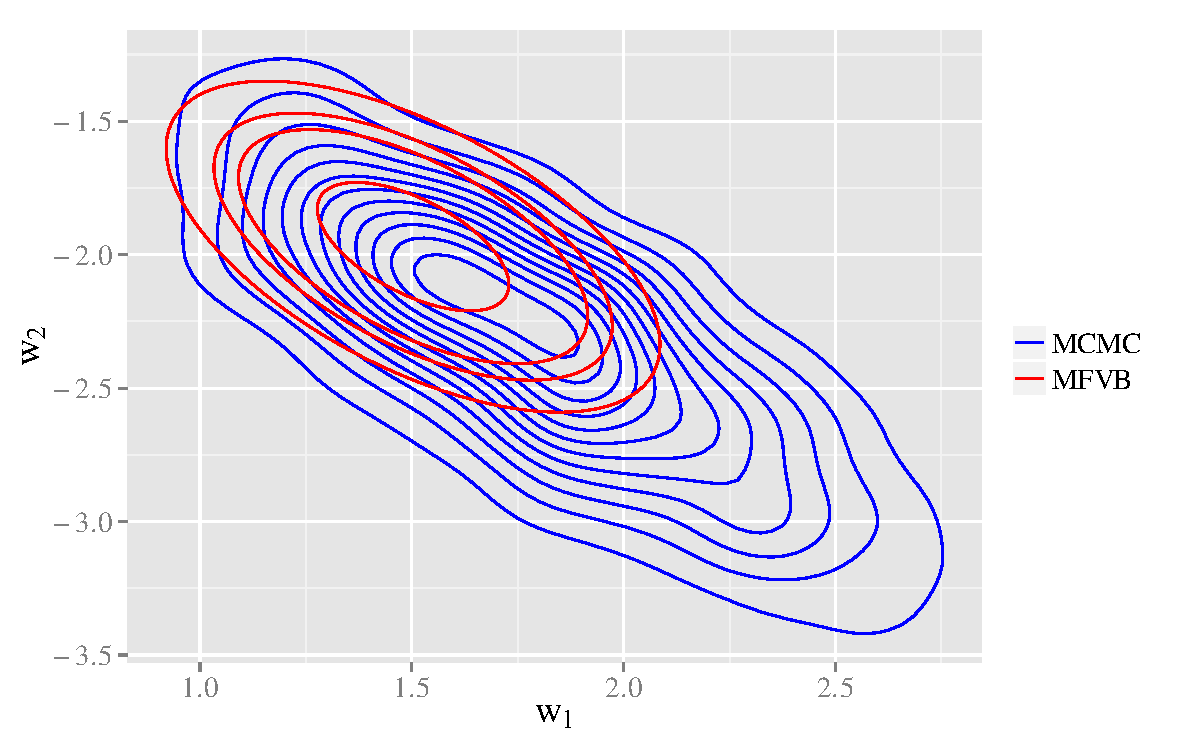
\includegraphics[height=100mm]{figures/mcmc_uniform_mfvb.pdf}
    \caption{Comparison of logistic regression point estimate, kernel density plot of MCMC simulations, and posterior density of
    MFVB logistic regression (vectorized function), for Dataset 0.   Contours of MFVB logistic regression indicate
    50\%, 90\%, 95\%, and 99\% confidence intervals for the bivariate normal $\mathcal{N}(\M{w}_{N},\M{V}_N)$.
    Mean values for MCMC and MFVB are also included.}  \label{fig:mcmc_mfvb}  
\end{figure}